\documentclass[onecolumn, draftclsnofoot,10pt, compsoc]{IEEEtran}
\usepackage{graphicx}
\usepackage{url}
\usepackage{setspace}
\usepackage{wrapfig}
\usepackage{indentfirst}


\usepackage{geometry}
\geometry{textheight=9.5in, textwidth=7in}

% 1. Fill in these details
\def \CapstoneTeamName{		    The Apolloers}
\def \CapstoneTeamNumber{		49}
\def \GroupMemberOne{			Jonathan Ropp}
\def \GroupMemberTwo{			Shannon Sandy}
\def \GroupMemberThree{			Dean Akin}
\def \CapstoneProjectName{		Apollo 11 3D Animation}
\def \CapstoneSponsorCompany{	OMSI}
\def \CapstoneSponsorPersona{	Jim Todd}
\def \CapstoneSponsorPersonb{	Mike Bailey}

% 2. Uncomment the appropriate line below so that the document type works
\def \DocType{		
                %Problem Statement
				%Requirements Document Draft
				%Technology Review
				%Design Document
				Progress Report
				}
			
\newcommand{\NameSigPair}[1]{\par
\makebox[2.75in][r]{#1} \hfil 	\makebox[3.25in]{\makebox[2.25in]{\hrulefill} \hfill		\makebox[.75in]{\hrulefill}}
\par\vspace{-12pt} \textit{\tiny\noindent
\makebox[2.75in]{} \hfil		\makebox[3.25in]{\makebox[2.25in][r]{Signature} \hfill	\makebox[.75in][r]{Date}}}}
% 3. If the document is not to be signed, uncomment the RENEWcommand below
\renewcommand{\NameSigPair}[1]{#1}

%%%%%%%%%%%%%%%%%%%%%%%%%%%%%%%%%%%%%%%
\begin{document}
\begin{titlepage}
    \pagenumbering{gobble}
    \begin{singlespace}
        \hfill 
        % 4. If you have a logo, use this includegraphics command to put it on the coversheet.
        
\includegraphics[height=4cm]{OSU_horizontal_2C_O_over_B.eps}   
        \par\vspace{.2in}
        \centering
        \scshape{
            \huge CS Capstone \DocType \par
            {\large\today}\par
            \vspace{.5in}
            \textbf{\Huge\CapstoneProjectName}\par
            \vfill
            {\large Prepared for}\par
            \Huge \CapstoneSponsorCompany\par
            \vspace{5pt}
            {\Large\NameSigPair{\CapstoneSponsorPersona}\par}
            {\Large\NameSigPair{\CapstoneSponsorPersonb}\par}
            {\large Prepared by }\par
            Group\CapstoneTeamNumber\par
            % 5. comment out the line below this one if you do not wish to name your team
            \CapstoneTeamName\par 
            \vspace{5pt}
            {\Large
                \NameSigPair{\GroupMemberOne}\par
                \NameSigPair{\GroupMemberTwo}\par
                \NameSigPair{\GroupMemberThree}\par
            }
            \vspace{20pt}
        }
        \begin{abstract}
        % 6. Fill in your abstract   
    
During this Winter term, our group has worked on creating a 3D animation for the Apollo 11 Moon Landing that will be shown in a planetarium at OMSI. We were finally able to meet Jim Todd in person and we changed some of our main goals of the project. Currently, the animation has reached beta functionality for the engineering expo and our next focus will be to prepare the animation for use in the planetarium. 

        \end{abstract}     
    \end{singlespace}
\end{titlepage}
\newpage
\pagenumbering{arabic}
\tableofcontents

% 7. uncomment this (if applicable). Consider adding a page break.
%\listoffigures
%\listoftables
\clearpage

% 8. now you write!

\section{Updated Goals}

%\begin{wrapfigure}{r}{0.5\textwidth}
    %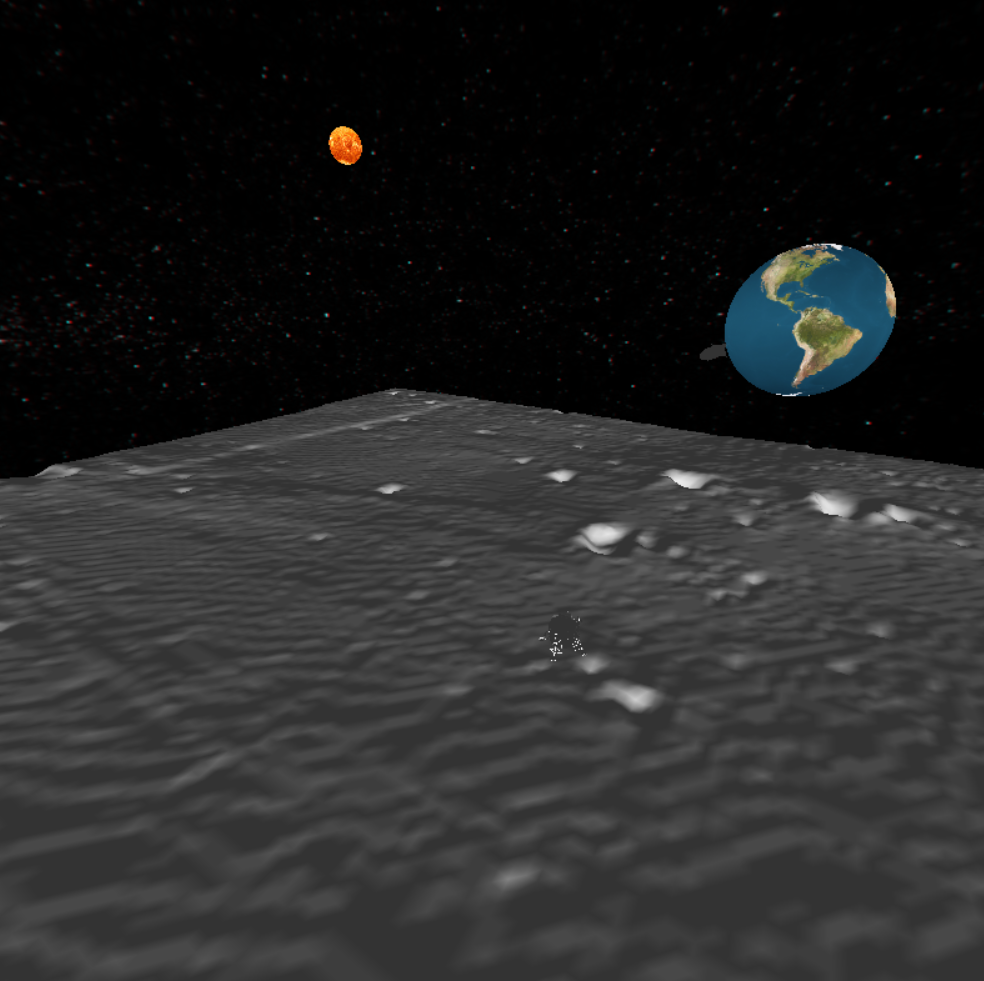
\includegraphics[width=0.5\textwidth]{View1.eps}
    %\caption{Apollo 11 Alpha - View 1: Lunar Surface}
    %\label{fig:View 1}
%\end{wrapfigure}

On January 3rd, our design group traveled to OMSI with Mike Bailey to meet with our client, Jim Todd, in person for the first time. We were treated to a full tour of the Harry C. Kendall Planetarium at the Oregon Museum of Science and Industry (OMSI) and got to see the inner workings of their setup. We learned that the planetarium received a software upgrade about a year ago and now uses DigitalSky: Dark Matter, a software produced by SkySkan, a provider of planetarium equipment and services. Jim showed us the Dark Matter interface on the main control computer and we got to see many different sample videos. This gave us a much better idea of how our project would look on a domed theater and how to best design the project to make the best use of the theater, as well as re-defining some of our goals. 

At the time of our visit, our group's plan was to animate all portions of the Apollo 11 mission, from launch to splashdown. However, when talking with Jim, we changed course to instead focus more on what happened on the Moon's surface and instead use original news footage to depict what happened before and after. We have some creative freedom with specifics, but our current story board is now as follows: 

\begin{itemize}
    \item The animation will start a view of the flight path of the Apollo 11 Command Module, including audio/video snippets of relevant quotes, and then when the module reaches the Moon, the decent of the Lunar Lander will be shown from the lunar surface.
    
    \item On the lunar surface, the operator will be able to change the view of the camera on the lunar surface. Key views will include the view of the Earth, a pan of the landscape, the American flag on the surface, and the Lunar Module During this time, the operator of the planetarium will be able to take questions from the audience and change the view accordingly. 
    
    \item When the operator is ready to bring the animation to an end, the Lunar Lander will be shown ascending from the lunar surface, then show the flight path again, again including audio/video clips from the mission. Lastly, credits will be displayed. 
    
\end{itemize}

Our group will implement this animation in OpenGL for the engineering expo and then translate it to a unique scripting language for use at the planetarium at OMSI. Some functionality, such as including historic video, will not be a feasible accomplishment for the OpenGL program, but from what we learned from Jim, this should be possible using the Dark Matter planetarium software at OMSI. Mike Bailey has been, and is currently in contact with Jim Todd as well as a contact with SkySkan to find the best ways to complete this conversion. At the end of this term, we are going to visit Jim Todd at OMSI and take a sample Dark Matter script with us to test in the planetarium. This will be a great indicator to if we are on the right track for getting an animation running in the planetarium. 

\section{Current Progress}
% Make it sound like we did a ton of work (Which we did!)

As of March 18th, our team has created a beta-level program in OpenGL that has the main scene of the Apollo 11 mission on the lunar surface. The lunar surface is placed at the origin and has the lunar module, an astronaut, and an American flag placed on the surface. These objects have been obtained from NASA's 3D object repository online except for the flag, which we modeled. The Moon and the Earth are included in the scene with a star map making up the background. We were able to accurately position and scale the Moon and Earth based on real measurements. 

Currently, there are seven viewpoints highlighting different views of the animation. These viewpoints include a diagram of the Apollo 11 flight path, Tranquility Base on the Moon, the Lunar module, flag, and astronaut, a view of the Earth from the Moon, and more. These views are bound to the number keys on a keyboard to change between them. Creating these views includes determining the position of the 'eye', where the eye should look, and the orientation of the eye, all in XYZ coordinates. 

In addition to the static views above, some views move throughout the scene. Panning across the lunar landscape and watching the Lunar Module descend to the surface are also included, with more being worked on now. These have been made using key-frame animation, where the eye-position moves between determined points in the scene. Also included with some views are audio snippets of notable quotes during the mission. These clips were chosen because they were either recognisable, or were directly related to the view. 

Our team scaled the lunar module, lunar surface, astronaut, and flag to make the scene look more realistic. The location of Tranquility Base is also marked on the Moon in a viewpoint to add context about where the Apollo 11 crew landed on the moon. We also reviewed historical photographs of the moon landing in order place the lunar module and American flag objects in the correct locations.
%Flight path
%Placement of objects
%lighting - Dean, you probably can write the best for this part
%shaders on the Earth - Dean, you again XD

\section{To Do}

From alpha to beta, we needed to add movement to the scene, which we did through animated views. The current views will be fine-tuned and more views will be added throughout the coming term. The majority of the presentation at OMSI will need to be in motion, with very few static views. In addition, the flight path will need to be animated with the Command Module traveling to and from the Moon. 

The majority of the OpenGL program is finished and ready for the engineering expo. That means that the remaining time will be focused on creating the presentation that will be shown in the planetarium at OMSI. Our current animation will need to be translated to a unique scripting language for use on the domed projection screen. This could result in issues due to the fact that we do not have the capability to test the Dark Matter script on our computers. We will decide a viable testing method during our next meeting with Jim Todd, but we will likely send Jim a script to test every other week, with Jim reporting on how it performed. 

%Something more here?

\section{Problems and Solutions}

One of the problems our group has encountered obtaining quality 3D objects for our scene. We found that NASA has a GitHub repository that contains .stl files for 3D objects from most of their missions. We obtained the models for the lunar module, astronaut, and lunar surface. However, these models were not to scale, so our group is continuing to adjust their sizes so they are more accurate. Another issue was that textures for the objects were ether incomplete or nonexistent. Recently, Mike Bailey decided that we needed better quality objects to show at expo, so he purchased high-quality models of the command module and lunar module. Changes to our program were necessary to load in the files, but it was well worth it. In addition, for the show at OMSI, Jim Todd should have access to other high-quality models as well.  

Another problem our group has encountered was integrating audio and video into our OpenGl project. For audio, the API we were planning on using uses a heavily deprecated library and the functions to play audio were not working. Instead, our group is currently using a Windows function to play audio files, making it so only computers with Windows OS can play audio. As for video, deprecated libraries were also the culprit, but after talking with Mike Bailey, we decided that our time would be better spent on improving the animation in other areas. For the presentation at OMSI, we are confident that audio and video will not be an issue, so to work towards that end, we are continuing to gather sources for the media. 

Lastly, a more general issue our group encountered was that SkySkan, the company that created the planetarium software, informed us that OpenGL is not directly compatible with their software. We have still decided that creating an OpenGL animation will be a requirement so that we can show something at the engineering expo. While making the animation compatible with the planetarium is still our main focus, for the purposes of priorities, we have moved that to become a stretch goal. That stretch goal is to convert our OpenGL program to a unique scripting language used by the planetarium's software. This should be just like learning a new coding language, but there may also be different functionalities that our team will need to learn and utilize. 

\section{Conclusion}

Our 3D animation of the Apollo 11 Mission is nearly ready for the Engineering Expo. Fine-tuning and additional animation will be all that is needed, but there is much to do for presentation at OMSI. The coming term will center around transferring our current animation to be able to be shown in OMSI's domed planetarium. Our upcoming meeting with Jim Todd should give us the final requirements for this project and more detailed goals for playing our animation at OMSI. 

\end{document}
